\section{A sharp Gamma translation theorem and explicit zeta identities}
\label{sec:gamma}

The first spectral derivative already gives a concrete identity tying
together an ordinary quadratic Gamma integral, polylogarithm order
derivatives, negative Hurwitz jets, and the first Stieltjes constant.
Define the periodic translation energy
\begin{equation}\label{eq:V-def}
 V(h)=\int_0^1
   \bigl[\log\Gamma(\{x+h\})-\log\Gamma(x)\bigr]^2\,dx,
 \qquad 0<h<1.
\end{equation}
The singularities are logarithmic and the integral converges ordinarily.
We extend it continuously by $V(0)=V(1)=0$.

\subsection{Three exact representations}

Put $Z_j(h)=\zeta^{(j)}(-1,h)+\zeta^{(j)}(-1,1-h)
-2\zeta^{(j)}(-1)$. Since $Z_0(h)=h(1-h)$, differentiation of
Theorem~\ref{thm:translation} yields the following explicit formula.

\begin{theorem}[Gamma--Hurwitz--polylogarithm identity]\label{thm:gamma-id}
For $0<h<1$,
\begin{equation}\label{eq:gamma-hurwitz}
 \boxed{\quad V(h)=Z_2(h)+2Z_1(h)
                  +\left(2+\frac{\pi^2}{3}\right)h(1-h).\quad}
\end{equation}
Equivalently, set $c=\gamma+\log(2\pi)$ and
\[
 E_j(h)=\zeta^{(j)}(2)-
       \Re\left.\partial_s^j\Li_s(e^{2\pi ih})\right|_{s=2}.
\]
Then
\begin{equation}\label{eq:gamma-polylog}
 V(h)=\frac{(c^2+\pi^2/4)E_0(h)-2cE_1(h)+E_2(h)}{\pi^2}.
\end{equation}
The following positive-odd-order series also converges for $0<h<1$:
\begin{align}
 V(h)&=h\left(\log^2h-2\log h+2+\frac{\pi^2}{3}\right)
          +\left(2\gamma_1-\frac{\pi^2}{3}\right)h^2\notag\\
 &\quad-\sum_{j=2}^{\infty}
    \frac{2\bigl[\zeta'(2j-1)+H_{2j-2}\zeta(2j-1)\bigr]}
         {j(2j-1)}h^{2j}.
 \label{eq:gamma-series}
\end{align}
Here $H_m=\sum_{k=1}^m1/k$ and $\gamma_1=\gamma_1(1)$.
\end{theorem}

\begin{proof}
From \eqref{eq:logR}, $\mathcal R_s(0,0)=\mathcal R_t(0,0)=1$
and $\mathcal R_{st}(0,0)=2+\pi^2/3$.
Thus \eqref{eq:translation-jets} with $r=q=1$ is exactly
\eqref{eq:gamma-hurwitz}. Formula \eqref{eq:gamma-polylog} follows
either by differentiating \eqref{eq:polylog-master} or directly from
\[
 \widehat{F_1}(k)=
 \frac{\gamma+\log(2\pi ik)}{2\pi ik}.
\]
The order derivatives of $\Li_s$ are legitimate here because the
corresponding series $\sum (\log k)^j/k^2$ converges absolutely.

For the series, use \eqref{eq:convergent-expansion}. At $j=1$,
\[
 u(u-1)\zeta(1+u)
  =-1+(1-\gamma)u+(\gamma+\gamma_1)u^2+O(u^3).
\]
The mixed derivative of this expression times $\mathcal R$ is
$2\gamma_1-\pi^2/3$. For $j\geq2$,
\[
 (u-1)_{2j}=-(2j-2)!\,u
       \bigl[1+(H_{2j-2}-1)u+O(u^2)\bigr].
\]
Multiplying by $\zeta(2j-1+u)$ and taking the mixed derivative
after multiplication by $\mathcal R$ gives
$-4[\zeta'(2j-1)+H_{2j-2}\zeta(2j-1)]/((2j)(2j-1))$.
The first term is \eqref{eq:P11}. This proves \eqref{eq:gamma-series}.
\end{proof}

\subsection{Strict concavity and the optimal translation}

\begin{theorem}[Sharp half-period maximum]\label{thm:gamma-max}
The function $V$ is strictly concave on $(0,1)$ and symmetric about
$1/2$. Its unique maximum is at $h=1/2$, with exact value
\begin{align}
 V_*={}&-3\zeta''(-1)+(2\log2-6)\zeta'(-1)
       -\frac{\log^22+2\log2}{12}+\frac12+\frac{\pi^2}{12}.
 \label{eq:Vmax}
\end{align}
In particular $V(h)\leq V_*$ for every real periodic shift $h$,
with equality exactly at $h\equiv1/2\pmod1$.
Numerically, $V_*=2.680722487980507384821524139517\ldots$.
\end{theorem}

\begin{figure}[tbp]
\centering
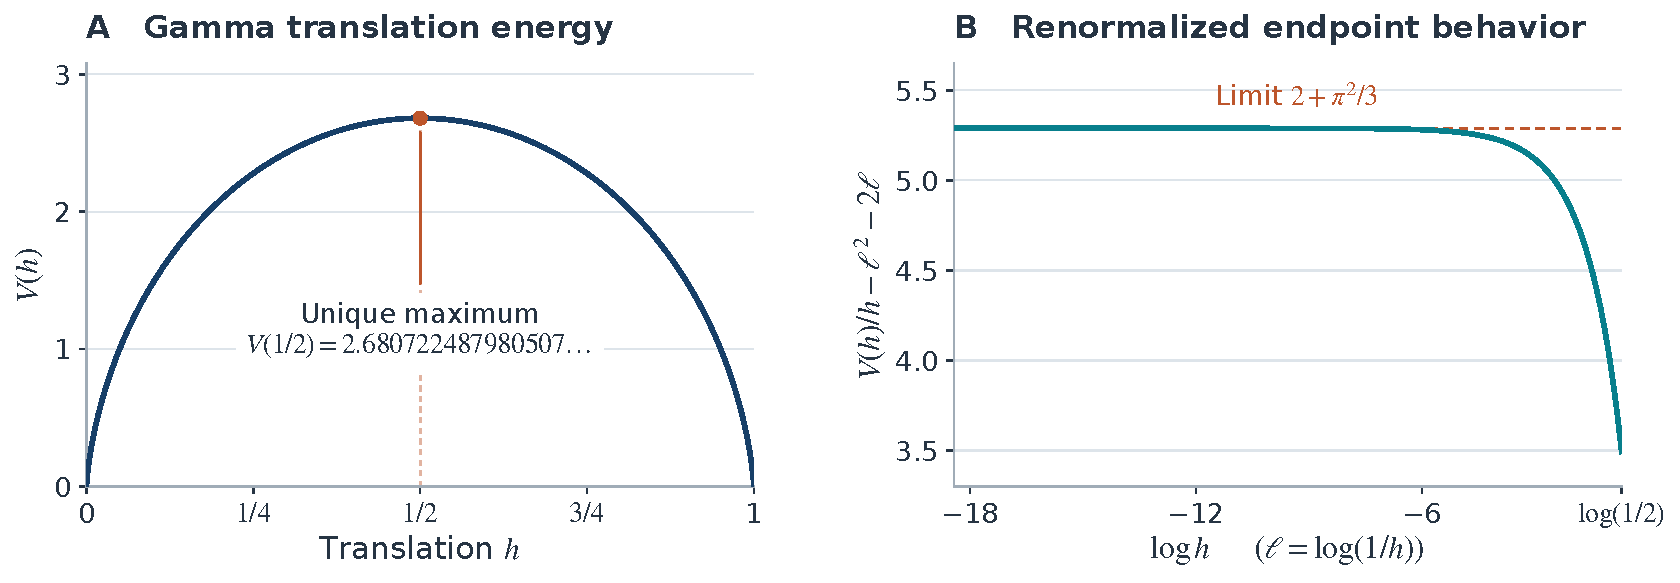
\includegraphics[width=\textwidth]{figures/gamma_translation.pdf}
\caption{The Gamma translation energy and its renormalized endpoint
limit. The left panel illustrates the proved strict concavity and
half-period maximum. The right subtracts the explicit logarithmic
terms, leaving a limit of $2+\pi^2/3$. Curves are evaluated from
the convergent series with its analytic truncation bound.}
\label{fig:gamma-energy}
\end{figure}

\begin{proof}
Twice differentiating \eqref{eq:gamma-hurwitz}, using the Laurent
expansion at $1$ before evaluating removable singularities, gives
\begin{equation}\label{eq:Vsecond}
 V''(h)=2\left(\gamma_1(h)+\gamma_1(1-h)-\frac{\pi^2}{3}\right).
\end{equation}
We prove a sufficient strict bound entirely analytically. The derivative
tower gives, by an absolutely convergent series,
\[
 \gamma_1'(a)=\sum_{m=0}^{\infty}
                 \frac{1-\log(m+a)}{(m+a)^2}.
\]
For $0<a\leq1$, its $m=0$ term is at least $1$, its $m=1$ term is
positive, and the possibly negative remaining terms have total magnitude
at most $\sum_{m\geq2}\log m/m^2$. The function $\log x/x^2$
is decreasing for $x\geq2$, so
\[
 -\zeta'(2)
 \leq\frac{\log2}{4}+\frac{\log3}{9}
         +\int_3^\infty\frac{\log x}{x^2}\,dx
 =\frac{\log2}{4}+\frac{4\log3}{9}+\frac13
 <\frac{359}{360}<1.
\]
The strict rational bound uses $\log2<7/10$ and $\log3<11/10$.
Hence $\gamma_1'(a)>0$ on $(0,1]$.

The sum-integral definition of $\gamma_1$, and decrease of
$\log x/x$ for $x\geq3$, also give
\[
 \gamma_1(1)
 \leq\frac{\log2}{2}+\frac{\log3}{3}
                         -\frac{\log^23}{2}
 <\frac{43}{60}<1<\frac{\pi^2}{6}.
\]
Thus both Stieltjes constants in \eqref{eq:Vsecond} are less than
$\pi^2/6$, proving strict concavity. Periodic translation invariance
gives $V(1-h)=V(h)$, so the unique maximum is at $1/2$.
Finally insert $\zeta(s,1/2)=(2^s-1)\zeta(s)$ and its first two
order derivatives into \eqref{eq:gamma-hurwitz}. This gives
\eqref{eq:Vmax}. The displayed decimal is a diagnostic evaluation;
neither the sign proof nor optimality depends on it.
\end{proof}

\subsection{Explicit derivatives, polygamma forms, and a definite primitive}

The exact Gamma energy also has useful identities beyond its second
derivative. For every integer $m\geq1$ and $0<h<1$,
\begin{equation}\label{eq:V-higher}
 V^{(m+2)}(h)=2\bigl[\gamma_1^{(m)}(h)
                         +(-1)^m\gamma_1^{(m)}(1-h)\bigr].
\end{equation}
The classical derivative tower takes the particularly simple form
\begin{equation}\label{eq:gamma1-polygamma}
 \gamma_1^{(m)}(a)=(-1)^{m+1}m!\zeta'(m+1,a)
                         +H_m\psi^{(m)}(a),\qquad a>0.
\end{equation}
Indeed, compare the coefficient of $u$ in
\[
 \partial_a^m\zeta(1+u,a)
 =(-1)^m(1+u)_m\zeta(m+1+u,a),
\]
using $\partial_u(1+u)_m|_{u=0}=m!H_m$ and
$\psi^{(m)}(a)=(-1)^{m+1}m!\zeta(m+1,a)$.
Equations \eqref{eq:V-higher}--\eqref{eq:gamma1-polygamma}
therefore express all higher shift derivatives directly in polygamma
functions and Hurwitz order derivatives at positive integers. The
identities apply on the open interval; the endpoint derivatives
generally diverge.

For the primitive, define
\[
 W_j(h)=\zeta^{(j)}(-2,h)-\zeta^{(j)}(-2,1-h),\qquad
 a_0=2+\frac{\pi^2}{3}.
\]
Corollary~\ref{cor:shift-primitive}, with $m=1$ followed by
$\partial_s\partial_t$ at zero, gives
\begin{align}
 \int_0^h V(v)\,dv={}&\frac{W_2(h)}2+\frac{3W_1(h)}2
            +\left(\frac74+\frac{\pi^2}{6}\right)W_0(h)\notag\\
 &-2h\bigl[\zeta''(-1)+2\zeta'(-1)+a_0\zeta(-1)\bigr].
 \label{eq:V-primitive}
\end{align}
There is no omitted integration constant: all $W_j$ vanish at zero
by continuous extension, since $h^2\log^j h\to0$. At $h=1$ this
becomes the exact mean-energy identity
\begin{equation}\label{eq:V-mean}
 \int_0^1 V(h)\,dh
 =-2\zeta''(-1)-4\zeta'(-1)+\frac13+\frac{\pi^2}{18}.
\end{equation}
It is also twice the centered second moment of $\log\Gamma$ on
$(0,1)$, as follows directly by averaging the defining translation.

\subsection{A convergent identity for the first Stieltjes constant}

The coefficients removed in \eqref{eq:gamma-series} are all positive.
Indeed, for $p\geq3$,
\[
 H_{p-1}\zeta(p)+\zeta'(p)
 \geq\frac32-\sum_{k\geq2}\frac{\log k}{k^3}
 \geq\frac32-\frac{\log2}{4}-\frac1{16}>0.
\]
They are $O(\log j/j^2)$ after the displayed prefactor in
\eqref{eq:gamma-series}. The series consequently extends uniformly to
$0\leq h\leq1$. Letting $h\uparrow1$ and using $V(1)=0$ proves
\begin{equation}\label{eq:gamma1-odd}
 \boxed{\quad
 \gamma_1=-1+\sum_{j=2}^{\infty}
   \frac{\zeta'(2j-1)+H_{2j-2}\zeta(2j-1)}{j(2j-1)}.
 \quad}
\end{equation}
This form is slow but has positive summands. Subtracting the elementary
harmonic contribution makes it geometrically convergent.

\begin{corollary}[An accelerated odd-zeta identity]\label{cor:gamma1-fast}
One has
\begin{equation}\label{eq:gamma1-fast}
 \boxed{\quad
 \gamma_1=2\log2-\log^22-1+
 \sum_{j=2}^{\infty}
 \frac{\zeta'(2j-1)+H_{2j-2}(\zeta(2j-1)-1)}{j(2j-1)}.
 \quad}
\end{equation}
If the sum is truncated at $j=J\geq2$, the absolute tail is bounded by
\begin{equation}\label{eq:gamma1-tail}
 \frac{16}{3}\,
 \frac{2+\log(2J+2)}{(J+1)^2}\,4^{-(J+1)}.
\end{equation}
\end{corollary}

\begin{proof}
The even part of $\sum_{n\geq0}H_nx^n=-\log(1-x)/(1-x)$ gives
\begin{align*}
 \sum_{j=2}^{\infty}\frac{H_{2j-2}}{j(2j-1)}
 &=2\int_0^1(1-x)\sum_{m\geq1}H_{2m}x^{2m}\,dx\\
 &=-\int_0^1\log(1-x)\,dx
     -\int_0^1\frac{1-x}{1+x}\log(1+x)\,dx\\
 &=2\log2-\log^22.
\end{align*}
Tonelli or absolute convergence justifies the interchange. Subtract
this value from \eqref{eq:gamma1-odd}.

For $p\geq3$, integral comparison yields
\[
 \zeta(p)-1\leq2^{1-p},\qquad
 |\zeta'(p)|\leq2\cdot2^{-p}.
\]
Together with $H_{2j-2}\leq1+\log(2j-2)$, each absolute summand
in the accelerated series is at most
$4(2+\log(2j))4^{-j}/j^2$. The factor
$(2+\log(2j))/j^2$ decreases, and summing the geometric tail gives
\eqref{eq:gamma1-tail}.
\end{proof}

For actual evaluation this tail bound is combined with controlled
evaluation of the finitely many zeta values and derivatives. A small
formal tail alone does not certify floating-point special-function
evaluations. The accompanying program explicitly labels its numerical
comparisons as diagnostics.

The same positivity gives useful global estimates. If
$A(h)=h(\log^2h-2\log h+2+\pi^2/3)
 +(2\gamma_1-\pi^2/3)h^2$, then
\begin{equation}\label{eq:V-bounds}
 A(h)-2(1+\gamma_1)h^4
 \leq V(h)\leq
 A(h)-\frac{\zeta'(3)+\tfrac32\zeta(3)}{3}h^4,
 \qquad 0<h<1.
\end{equation}
The left inequality is sharp at $h=1$ by continuity, and the right
has the exact first omitted coefficient at zero. For computation one
may replace $h$ by $\min(h,1-h)$ before using the convergent series.
